\documentclass[
	11pt, % Set the default font size, options include: 8pt, 9pt, 10pt, 11pt, 12pt, 14pt, 17pt, 20pt
	t, % Uncomment to vertically align all slide content to the top of the slide, rather than the default centered
	% aspectratio=169, % Uncomment to set the aspect ratio to a 16:9 ratio which matches the aspect ratio of 1080p and 4K screens and projectors
        russian
]{beamer}

\graphicspath{{Images/}{./}}
\usepackage{booktabs} % Allows the use of \toprule, \midrule and \bottomrule for better rules in tables
\usepackage[russian]{babel}
\usepackage[dvipsnames]{xcolor}
\usepackage{xcolor}

% Beamer comes with a number of default layout themes which change the colors and layouts of slides. Below is a list of all themes available, uncomment each in turn to see what they look like.

% \usetheme{default}
%\usetheme{AnnArbor}
%\usetheme{Antibes}
%\usetheme{Bergen}
%\usetheme{Berkeley}
%\usetheme{Berlin}
%\usetheme{Boadilla}
%\usetheme{CambridgeUS}
%\usetheme{Copenhagen}
%\usetheme{Darmstadt}
%\usetheme{Dresden}
%\usetheme{Frankfurt}
%\usetheme{Goettingen}
%\usetheme{Hannover}
%\usetheme{Ilmenau}
%\usetheme{JuanLesPins}
%\usetheme{Luebeck}
\usetheme{Madrid}
%\usetheme{Malmoe}
%\usetheme{Marburg}
%\usetheme{Montpellier}
%\usetheme{PaloAlto}
%\usetheme{Pittsburgh}
%\usetheme{Rochester}
%\usetheme{Singapore}
%\usetheme{Szeged}
% \usetheme{Warsaw}

% Beamer comes with a number of color themes that can be applied to any layout theme to change its colors. Uncomment each of these in turn to see how they change the colors of your selected layout theme.

% \usecolortheme{spruce}
% \usecolortheme{whale}


\usefonttheme{default} % Typeset using the default sans serif font
%\usefonttheme{serif} % Typeset using the default serif font (make sure a sans font isn't being set as the default font if you use this option!)
%\usefonttheme{structurebold} % Typeset important structure text (titles, headlines, footlines, sidebar, etc) in bold
%\usefonttheme{structureitalicserif} % Typeset important structure text (titles, headlines, footlines, sidebar, etc) in italic serif
%\usefonttheme{structuresmallcapsserif} % Typeset important structure text (titles, headlines, footlines, sidebar, etc) in small caps serif
\usepackage{palatino} % Use the Palatino font for serif text
\usepackage[default]{opensans} % Use the Open Sans font for sans serif text
\usepackage{mathrsfs}
\usepackage{amsmath}
\useinnertheme{circles}
\useoutertheme{default}

%\setbeamertemplate{footline} % Uncomment this line to remove the footer line in all slides
%\setbeamertemplate{footline}[page number] % Uncomment this line to replace the footer line in all slides with a simple slide count

%\setbeamertemplate{navigation symbols}{} % Uncomment this line to remove the navigation symbols from the bottom of all slides

\title[]{Анализ смещения распределений в контрастивном обучении}
\author[Лидия Троешестова \and Роман Исаченко]{Лидия Троешестова \and Роман Исаченко}
\institute[]{Московский физико-технический институт}
\date[\today]{\today}


\begin{document}
\begin{frame}
	\titlepage % Output the title slide, automatically created using the text entered in the PRESENTATION INFORMATION block above
\end{frame}

\setbeamerfont{frametitle}{size=\small}
%------------------------------------------------

\begin{frame}
    \frametitle{Цель исследования}
\footnotesize
\begin{block}{ \small Цель}
Исследовать влияние смещения распределения $p_x^+$ в задаче построения представлений без учителя.
\end{block}

\begin{block}{ \small Проблема}
Наличие смещения в распределениях классов приводит к некорректным представлениям объектов.
\end{block}

\begin{block}{ \small Идея}
Учесть смещения распределений классов путем построения несмещенной функции потерь.
% Построить несмещенную функцию потерь, используя оценку распределения $p_x^+$ в предположении верности негативных объектов.
\end{block}

\begin{equation*} \small
L_{\text{Unbiased}}^N(f) = \mathbb{E}_{\substack{\mathbf{x} \sim p, \mathbf{x^+} \sim p^+_x,\\ \mathbf{x^-} \sim p_x^-}} \bigg[-\log \frac{\exp (\scriptsize\text{sim}_f(\mathbf{x}, \mathbf{x^+}))}{\exp (\scriptsize\text{sim}_f(\mathbf{x}, \mathbf{x^+}) + \sum _{i=1}^N \exp (\scriptsize\text{sim}_f(\mathbf{x}, \mathbf{x^-})}\bigg]
\end{equation*}

\end{frame}
%------------------------------------------------

\begin{frame}
    \frametitle{Смещение распределений при построении представлений}
\footnotesize
\begin{itemize}
    \item $p^+_x(\mathbf{x'})$ — вероятность взять $\mathbf{x'}$ как позитивный объект для $\mathbf{x}$.
    \item $p^-_x(\mathbf{x'})$ — вероятность взять $\mathbf{x'}$ как негативный объект для $\mathbf{x}$.
    \item $\tau^+$ — вероятность 1 класса;
    \item $\tau^- = 1 - \tau^+$ — вероятность любого другого класса
    \item $p(\mathbf{x'}) = \tau^+ p_x^+(\mathbf{x'}) + \tau^-p_x^-(\mathbf{x'})$
\end{itemize}

\begin{figure}
\centering
\begin{subfigure}
  \centering
  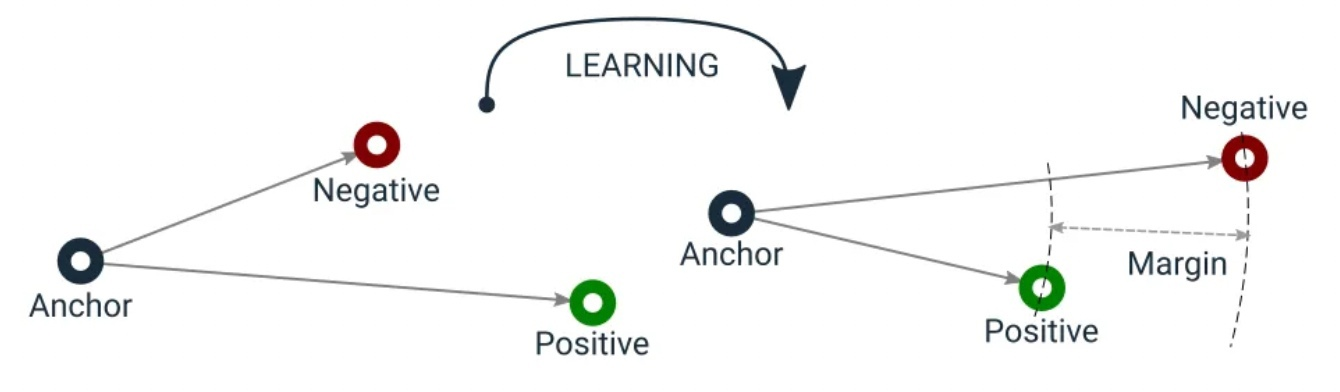
\includegraphics[width=.4\linewidth]{Images/triplet.jpeg}
  % \caption{Triplet loss visualization}
  \label{fig:sub1}
\end{subfigure}%
\begin{subfigure}
  \centering
  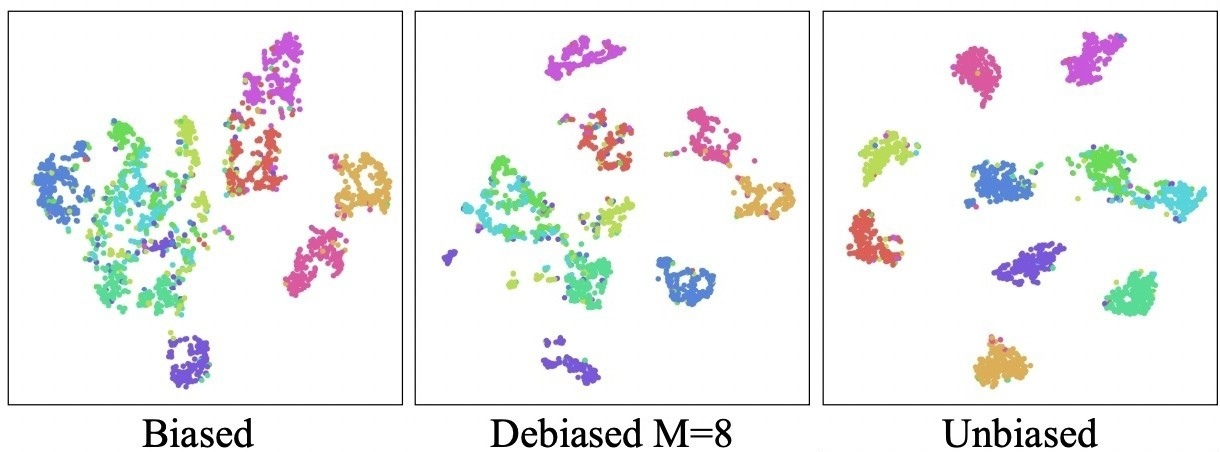
\includegraphics[width=.5\linewidth]{Images/t-SNE.jpeg}
  % \caption{t-SNE visualization of learned representations on CIFAR10}
  \label{fig:sub2}
\end{subfigure}
\label{fig:test}
\end{figure}

Найти $L_{\text{DebiasedPos}}^N$, минимизирующее $\lim \limits_{N \to \infty} \big|L_{\text{DebiasedPos}}^N (f)  - L_{\text{Unbiased}}^N(f)\big|$.

\begin{equation*} \small
L_{\text{Unbiased}}^N(f) = \mathbb{E}_{\substack{\mathbf{x} \sim p, \mathbf{x^+} \sim p^+_x,\\ \mathbf{x^-} \sim p_x^-}} \bigg[-\log \frac{\exp (\scriptsize\text{sim}_f(\mathbf{x}, \mathbf{x^+}))}{\exp (\scriptsize\text{sim}_f(\mathbf{x}, \mathbf{x^+}) + \sum _{i=1}^N \exp (\scriptsize\text{sim}_f(\mathbf{x}, \mathbf{x^-})}\bigg]
\end{equation*}

\end{frame}
%------------------------------------------------

\begin{frame} 
	\frametitle{Список литературы}
	
	\begin{thebibliography}{99} 
		\footnotesize
		
		\bibitem[Chuang, 2020]{p1}
			Ching-Yao Chuang, Joshua Robinson, Lin Yen-Chen, Antonio Torralba, Stefanie Jegelkah (2020)
			\newblock Debiased Contrastive Learning

            \bibitem[khosla2021supervised, 2020]{p2}
			Prannay Khosla, Piotr Teterwak, Chen Wang, Aaron Sarna, Yonglong Tian, Phillip Isola, Aaron Maschinot, Ce Liu, Dilip Krishnan (2021)
			\newblock Supervised Contrastive Learning

           \bibitem[Chen2020SimCLR, 2020]{p3}
			CTing Chen, Simon Kornblith, Mohammad Norouzi, Geoffrey Hinton (2020)
			\newblock A Simple Framework for Contrastive Learning of Visual Representations

   		\bibitem[Sohn, 2016]{p4}
			Sohn, Kihyuk (2016)
			\newblock Improved Deep Metric Learning with Multi-class N-pair Loss Objective

   		\bibitem[schroff2015facenet, 2015]{p5}
			Florian Schroff, Dmitry Kalenichenko, James Philbin (2015)
			\newblock FaceNet: A Unified Embedding for Face Recognition and Clustering

	\end{thebibliography}
\end{frame}
%------------------------------------------------

\begin{frame}
    \frametitle{Учет ошибок первого рода}
\scriptsize
Обозначим $h(\textbf{x}, \widetilde{\textbf{x}}) := e^{f(\textbf{x})^T f(\widetilde{\textbf{x}})}$.

\begin{lemma}
При $N \to \infty$:
\begin{equation*}
L_{\text{Unbiased}}^N(f) 
\longrightarrow
\mathbb{E}_{\substack{\textbf{x} \sim p \\ \textbf{x}^- \sim p_x^-}} \bigg[ - \log \frac{R}{R + N \color{blue} \mathbb{E}_{\textbf{x}^- \sim p_x^-} h(\textbf{x}, \textbf{x}^-)}\bigg],
\end{equation*}
где
\begin{equation*}
R = \frac{1}{\tau^+} \big(\color{violet} \mathbb{E}_{\textbf{x}' \sim p} h(\textbf{x}, \textbf{x}') \color{black}  - \tau^- \color{blue} \mathbb{E}_{\textbf{x}^- \sim p_x^-} h(\textbf{x}, \textbf{x}^-)\big).
\end{equation*}
\end{lemma}

\begin{equation*}
\tilde{L}_{\text{DebiasedPos}}^N (f) = \mathbb{E}_{\substack{\textbf{x} \sim p \\ \textbf{x}^- \sim p_x^-}} \bigg[ - \log \frac{\color{violet} \mathbb{E}_{\textbf{x}' \sim p} h(\textbf{x}, \textbf{x}') \color{black} - \tau^- \color{blue} \mathbb{E}_{\textbf{x}^- \sim p_x^-} h(\textbf{x}, \textbf{x}_i^-)}{\color{violet} \mathbb{E}_{\textbf{x}' \sim p} h(\textbf{x}, \textbf{x}') \color{black} + \big(N \tau^+ - \tau^-\big) \color{blue} \mathbb{E}_{\textbf{x}^- \sim p_x^-} h(\textbf{x}, \textbf{x}_i^-)}\bigg]
\end{equation*}

Оценим неизвестные матожидания эмпирически:
\begin{equation*}
\color{violet}P_{\text{emp}} (\textbf{x}, \{\textbf{u}_i\}_{i=1}^N, \textbf{v}) = \frac{1}{N+2} \bigg(\sum \limits_{i=1}^N h(\textbf{x}, \textbf{u}_i) + h(\textbf{x}, \textbf{v}) + h(\textbf{x}, \textbf{x})\bigg)\color{black}; \color{blue} P_{\text{emp}}^- (\textbf{x}, \{\textbf{u}_i\}_{i=1}^N) = \frac{1}{N} \sum \limits_{i=1}^N h(\textbf{x}, \textbf{u}_i).
\end{equation*}

\end{frame}
%------------------------------------------------

\begin{frame}
    \frametitle{Учет ошибок первого рода}
\scriptsize

\begin{equation*}
\tilde{L}_{\text{DebiasedPos}}^N (f) = \mathbb{E}_{\substack{\textbf{x} \sim p \\ \textbf{x}^- \sim p_x^-}} \bigg[ - \log \frac{\color{violet} \mathbb{E}_{\textbf{x}' \sim p} h(\textbf{x}, \textbf{x}') \color{black} - \tau^- \color{blue} \mathbb{E}_{\textbf{x}^- \sim p_x^-} h(\textbf{x}, \textbf{x}_i^-)}{\color{violet} \mathbb{E}_{\textbf{x}' \sim p} h(\textbf{x}, \textbf{x}') \color{black} + \big(N \tau^+ - \tau^-\big) \color{blue} \mathbb{E}_{\textbf{x}^- \sim p_x^-} h(\textbf{x}, \textbf{x}_i^-)}\bigg]
\end{equation*}

Финальная оценка:
\begin{equation*}
L_{\text{DebiasedPos}}^N (f) = \mathbb{E}_{\substack{\textbf{x} \sim p \\ \{\textbf{u}_i\}_{i=1}^N \sim {p_x^-}^N \\ \textbf{v} \sim p_x^+}} \bigg[-\log \frac{\color{violet}P_{\text{emp}} \color{black} - \tau^- \color{blue} P_{\text{emp}}^-} {\color{violet}P_{\text{emp}} \color{black} + \big(N \tau^+ - \tau^-\big) \color{blue} P_{\text{emp}}^- }\bigg].
\end{equation*}

\begin{theorem}
Для произвольного представления f и произвольного $\delta > 0$ существует достаточно большое $N$, что
\begin{equation*}
\big|\tilde{L}_{\text{DebiasedPos}}^N (f) - L_{\text{DebiasedPos}}^N (f)\big| \leq \bigg[\bigg(1 + \frac{\tau^-}{\tau^+} + \delta\bigg) \sqrt{\frac{\pi}{2N}} + \bigg(1 + \frac{1}{\tau^+}\bigg) \sqrt{\frac{\pi}{2N + 2}}\bigg] e^{3/2}
\end{equation*}
\end{theorem}

\end{frame}
%------------------------------------------------

\begin{frame}
	\frametitle{Использование SimCLR}
	\framesubtitle{CTing Chenet al., 2020} % Optional subtitle

\begin{figure}
    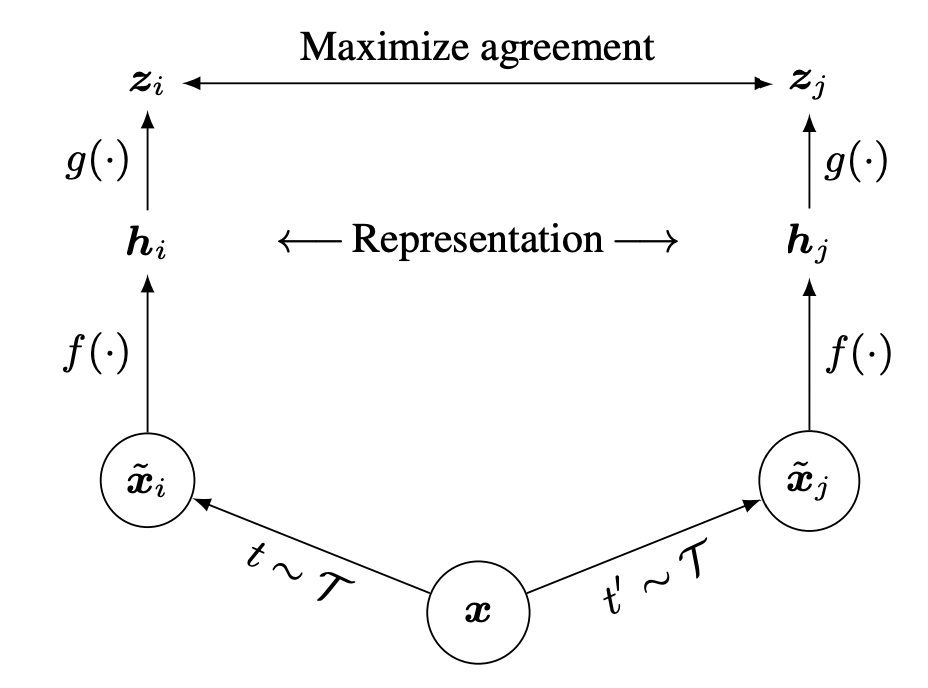
\includegraphics[width=0.5\linewidth]{Images/simclr.png}
\end{figure}

\scriptsize
\begin{itemize}
    \item $\mathcal{T} -$ семейство аугментаций (color distortion, Gaussian blur) 
    \item Семплируются 2 аугментации $t, t' \sim \mathcal{T}$, применяются к каждому объекту.
    \item Обучаем сеть-энкодер $f(\cdot)$ и MLP сеть-проекцию $g(\cdot)$, максимизируя соответствие представлений.
\end{itemize}
\end{frame}
%------------------------------------------------

\begin{frame}
	\frametitle{Вычислительный эксперимент}
\scriptsize

\begin{block}{ \small Цель эксперимента}
Сравнить качество представлений при использовании 3 функций потерь: Contrastive, DebiasedNeg и DebiasedPos. 
\end{block}

\begin{block}{ \small Обучение}
\begin{itemize}
    \item Обучаем SimCLR с энкодером ResNet-18 и оптимизатором Adam, 50 эпох с размером батча 512.
    \item Фиксируем выученные представления изображений из CIFAR10 на обучающей выборке.
\end{itemize}
\end{block}

\begin{block}{ \small Валидация}
На тестовой выборке классифицируем объект, применяя top-K к банку представлений, считаем top-1 и top-5 accuracy.
\end{block}

\end{frame}
%------------------------------------------------

\begin{frame}
    \frametitle{\small Эксперимент с удалением FN, эксперимент с добавлением FP}

\scriptsize
Функция потерь DebiasedPos устойчива к шуму и имеет превосходство на ранних эпохах.

\begin{figure}
\centering
\begin{subfigure}
  \centering
  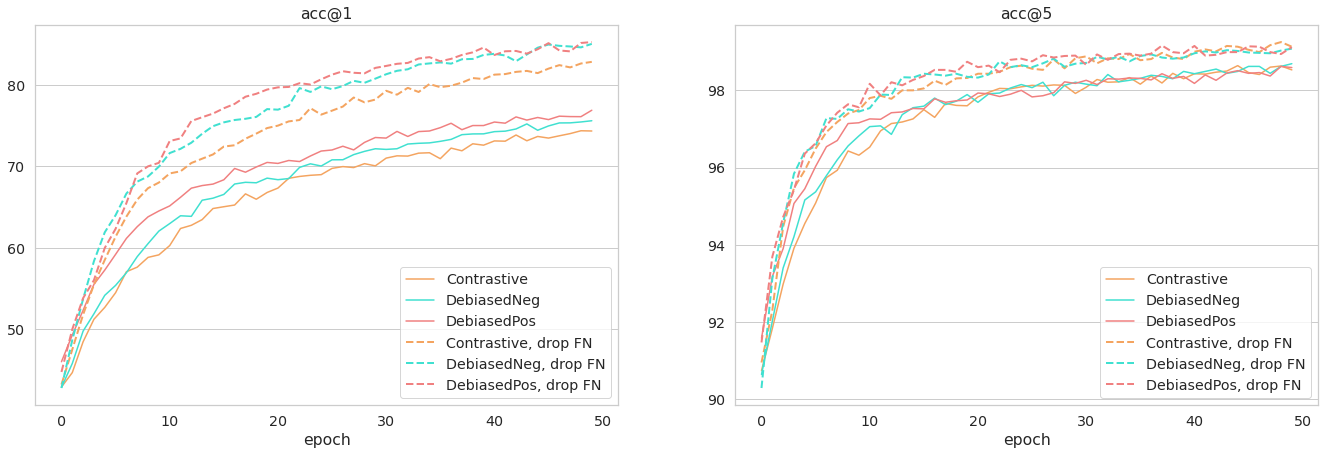
\includegraphics[width=0.87\linewidth]{Images/base_vs_dropfn.png}
  \label{fig:sub1}
\end{subfigure}%

\begin{subfigure}
  \centering
  \hspace*{+0.22cm}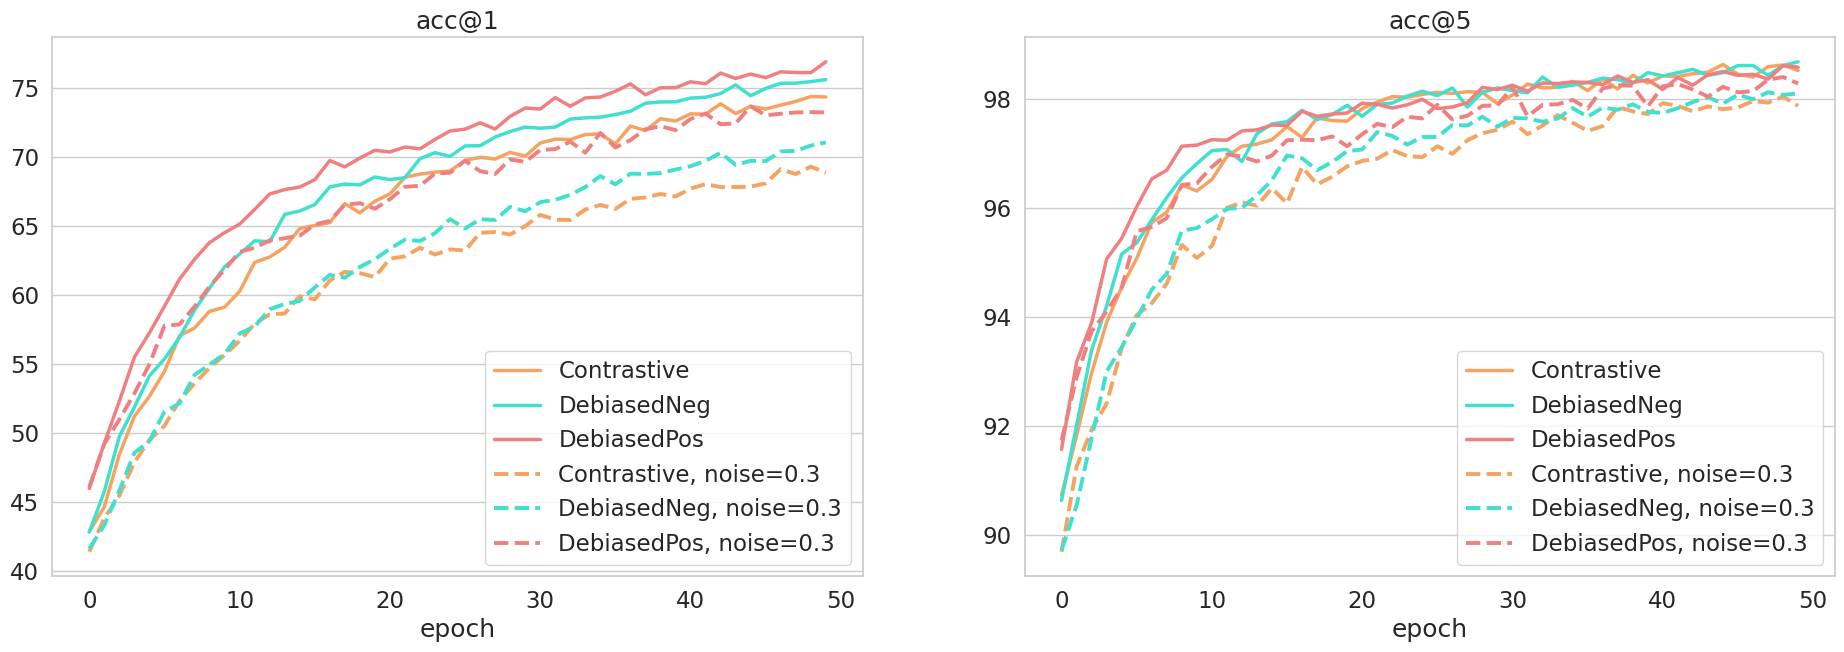
\includegraphics[width=0.87\linewidth]{Images/base_vs_noise.png}
  \label{fig:sub2}
\end{subfigure}
\label{fig:test}
\end{figure}


	
\end{frame}
%------------------------------------------------

\begin{frame}
	\frametitle{Увеличение кол-ва позитивных объектов $M$}
\scriptsize
Способы агрегации по $M$:
\begin{enumerate}
    \item \textit{pos-grouping}: внутри оценки $\color{violet}P_{\text{emp}} (\textbf{x}, \{\textbf{u}_i\}_{i=1}^N, \{\textbf{v}_j\}_{j=1}^M)$ вместо $h(\textbf{x}, \textbf{v})$ используем $\frac{1}{M} \sum \limits_{j=1}^M h(\textbf{x}, \textbf{v}_j)$.
    \item \textit{loss-combination}: для каждой пары позитивных объектов считаем $L_{\text{DebiasedPos}}^N (f)$ и берем среднее по всем значениям функции потерь.


\end{enumerate}

\begin{figure}
\centering
\begin{subfigure}
  \centering
  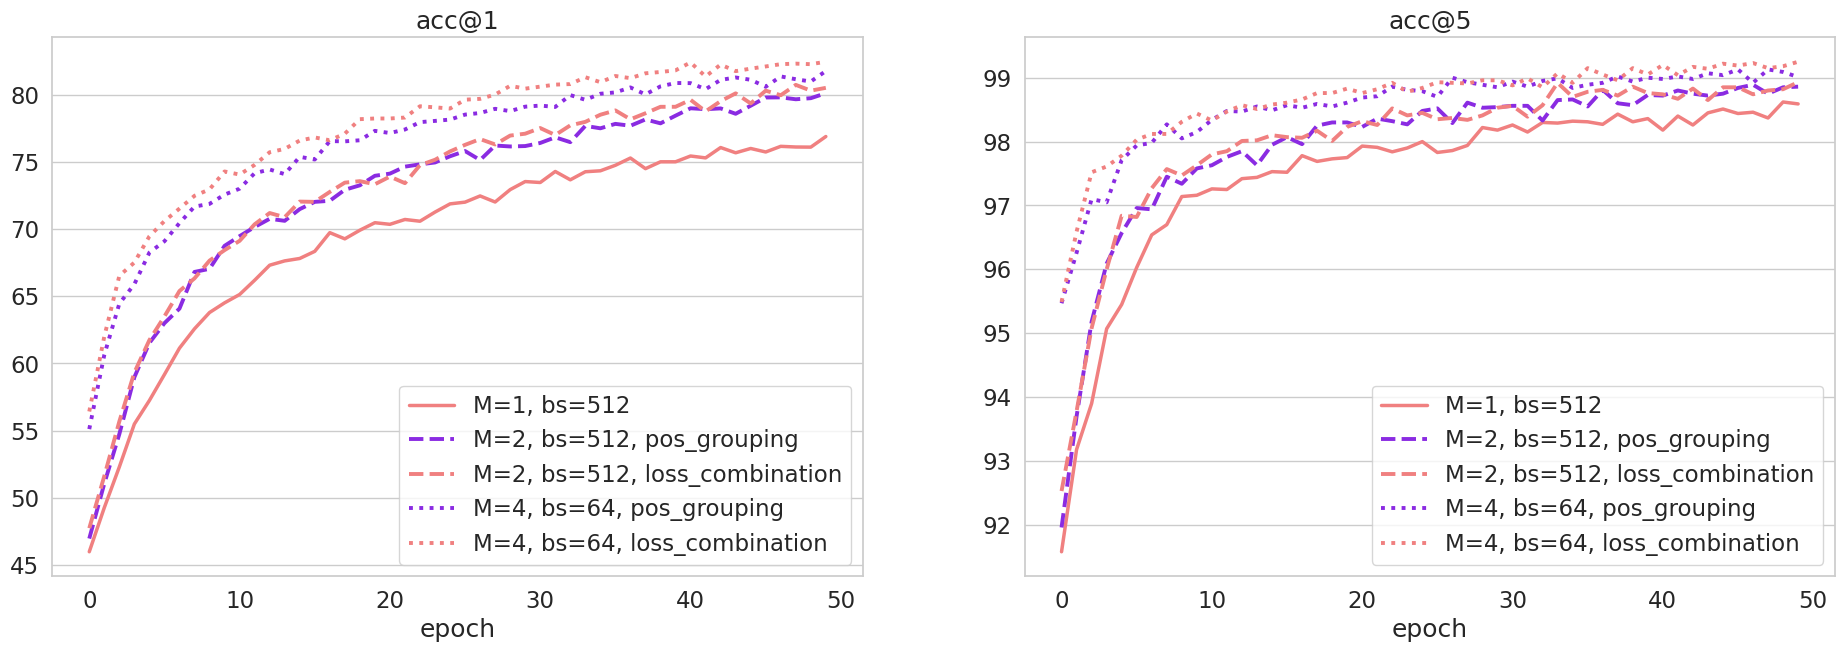
\includegraphics[width=1\linewidth]{Images/pg_vs_lc.png}
  \label{fig:sub1}
\end{subfigure}
\label{fig:test}
\end{figure}

\scriptsize При увеличении $M$ точность значительно возрастает, причем \textit{loss-combination} лучше, чем \textit{pos-grouping}.
	
\end{frame}

%------------------------------------------------

\begin{frame}
	\frametitle{Увеличение кол-ва позитивных объектов $M$}
\scriptsize
\begin{table}
    \tiny
    \centering
    \begin{tabular}{llllll}
        \toprule
        Method  & M & bs    & Training time (min)   & acc@1 & acc@5\\
        \midrule
        -   & 1 & 512   & 122.85    & 76.76 & 98.61\\
        \midrule
        pos-grouping    & 2 & 512   & \textbf{181.87}   & 80.1  & 98.86\\
        loss-combination    & 2 & 512   & 192.82    & \textbf{80.5} & \textbf{98.93}\\
        \midrule
        pos-grouping    & 4 & 64    & \textbf{278.88}   & 81.75 & 99.01\\
        loss-combination    & 4 & 64    & 308.25    & \textbf{82.44} & \textbf{99.25}\\
        \bottomrule
    \end{tabular}
    \label{tab:table}
\end{table}

\scriptsize Есть trade-off между производительностью и точностью.

\begin{figure}
\centering
\begin{subfigure}
  \centering
  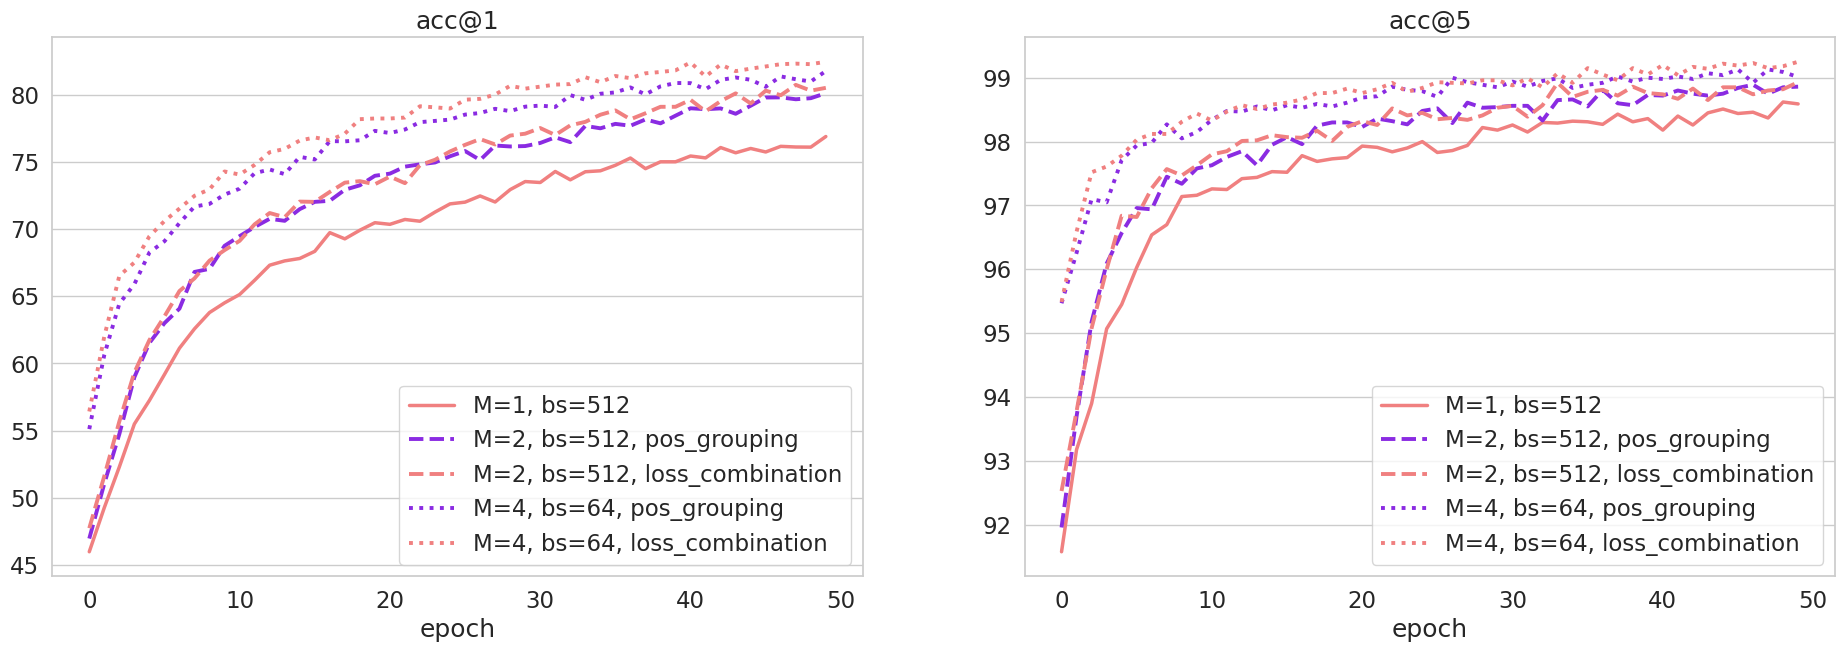
\includegraphics[width=1\linewidth]{Images/pg_vs_lc.png}
  \label{fig:sub1}
\end{subfigure}
\label{fig:test}
\end{figure}

\end{frame}

%------------------------------------------------

\begin{frame}
    \frametitle{Заключение}

\begin{itemize}
\small
    \item При верности предположения о правильности негативных объектов функция потерь DebiasedPos работает корректно.
    \vfill
    \item DebiasedPos более устойчив к шумным датасетам: когда увеличена доля ошибок I рода, DebiasedPos имеет большое преимущество в точности.
    \vfill
    \item При увеличенном кол-ве позитивных объектов точность для всех рассмотренных функций потерь возрастает.
    \vfill
    \item Способ агрегации \textit{pos-grouping} менее затратный, а \textit{loss-combination} более точный.
\end{itemize}

\end{frame}


\end{document} 